\subsubsection{Sichtfeld der Kamera}
\label{subsub:sichtfeld-der-kamera}
Damit sichergestellt werden kann dass die Kamera das gesamte Spielfeld fotografieren kann, wird in diesem Abschnitt das Sichtfeld der Kamera berechnet. Auf der Website von \citeauthor{raspberry-pi-camera} \citeyear{raspberry-pi-camera} wurden diverse Tests mit dem Raspberry Pi Camera Modul (siehe Abschnitt \ref{subsub:kamera}) durchgeführt. Diese haben ergeben dass die Kamera ein horizontales Sichtfeld von $53^\circ$ und ein vertikales Sichtfeld von $40^\circ$ hat. Wie man der Abbildung \ref{fig:berechnung_sichtfeld} entnehmen kann ergibt das bei einer Distanz von zwei Meter eine Aufnahmefläche von 2×1.3 Meter.

\begin{figure}[h!]
\centering
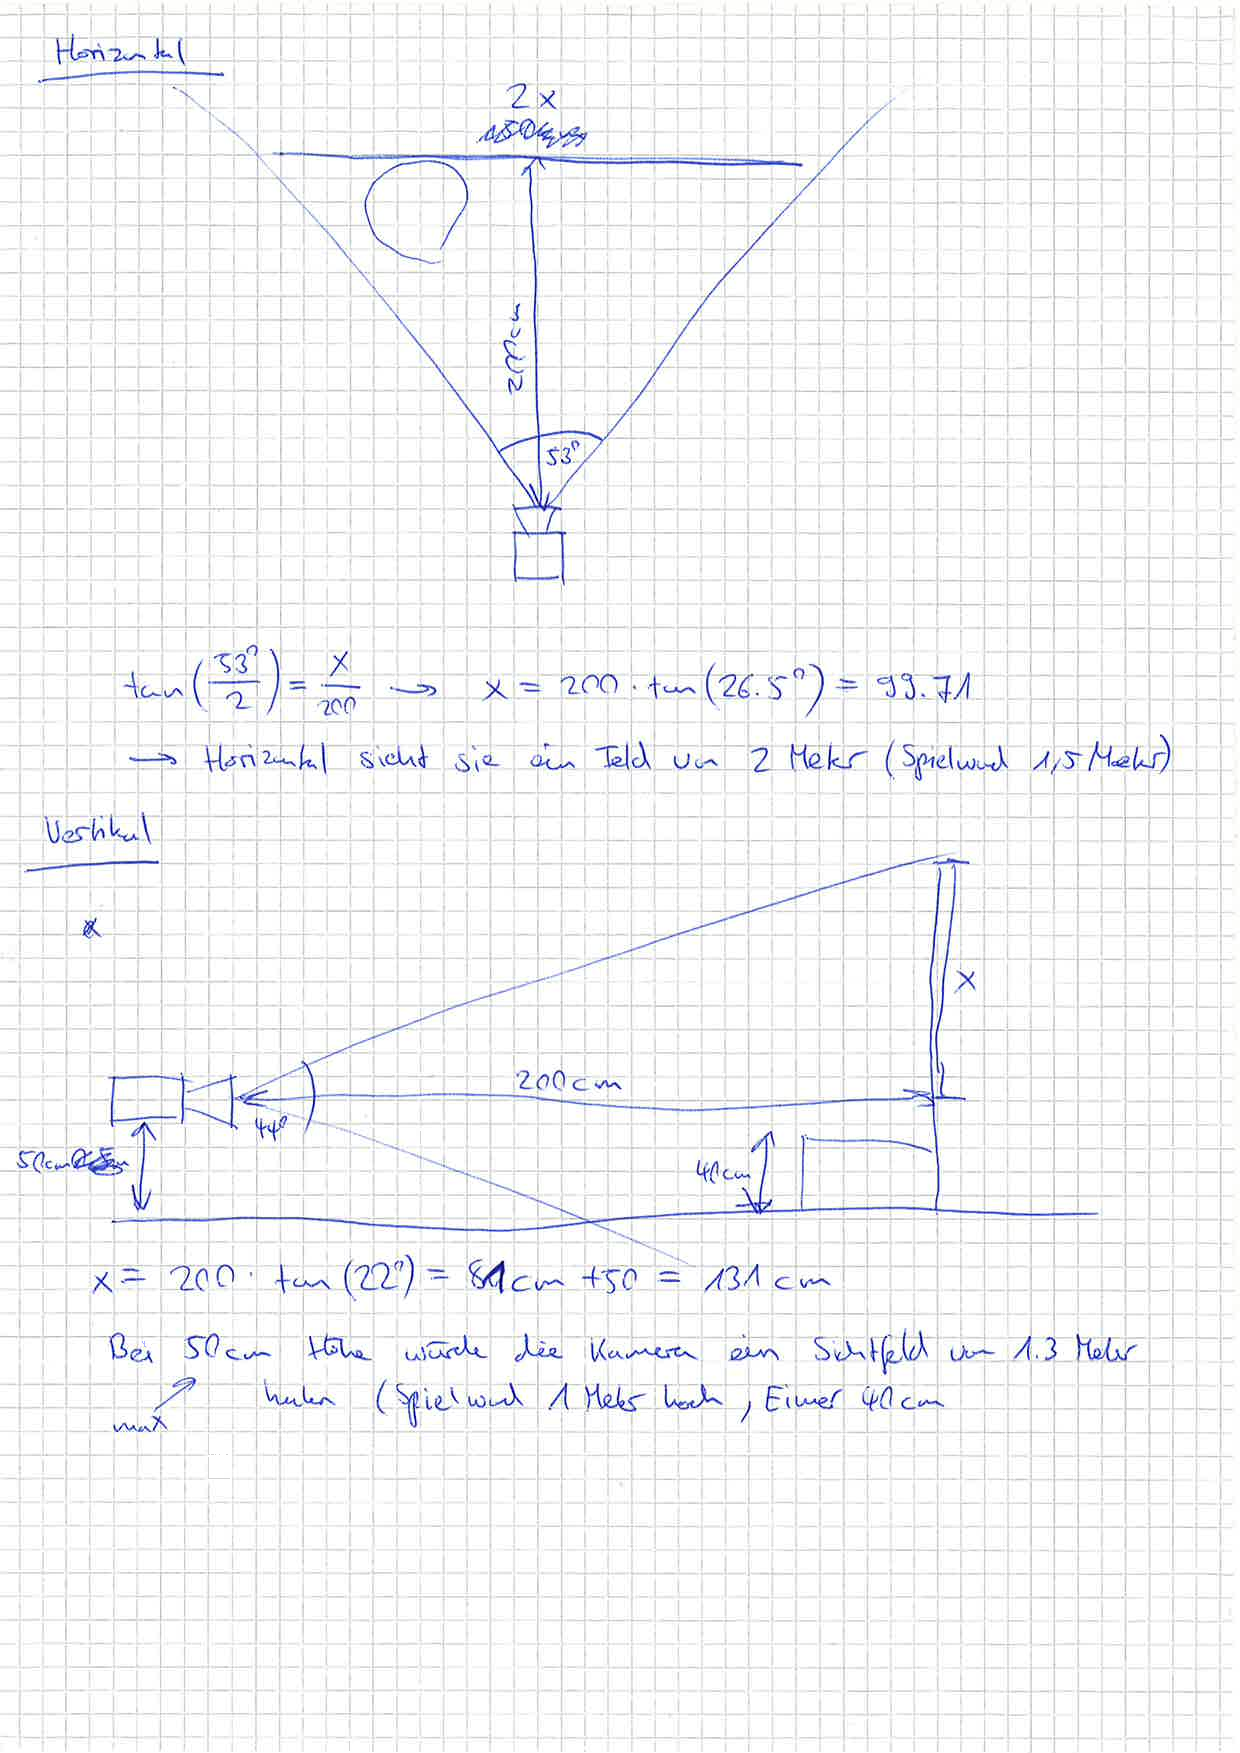
\includegraphics[width=0.7\linewidth]{../../fig/berechnung_sichtfeld.pdf}
\caption{Berechnung des Sichtfeldes der Kamera}
\label{fig:berechnung_sichtfeld}
\end{figure}
